
\newpage
\section{Casos de uso}
El la siguiente sección se define y describen los Actores,funciones y esenarios, describiendo su funcionalidad e interacción dentro de la aplicación.\par
\vspace{5mm}
\begin{figure}[h!]
	\centering
	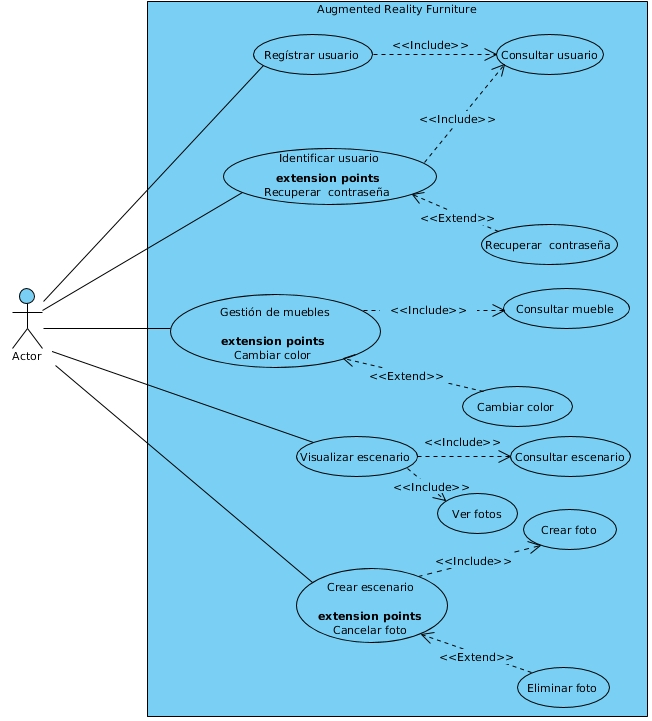
\includegraphics[width=15cm,height=17cm]{imagenes/analisis/casosDeUso.jpg}
	\caption{Casos de uso.}
	\label{fig:analogo}
\end{figure}  
\newpage

\subsection{Caso de uso 1} \textit{Login}\par
Escenario general para el acceso a la aplicación con un correo y una contraseña valida. Incluye una función que recupera la contraseña de los usuarios mediante el envío de su contraseña a su correo electrónico
\begin{figure}[h!]
	\centering
	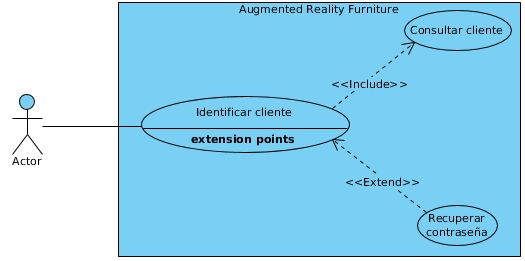
\includegraphics[width=12cm,height=6cm]{imagenes/analisis/login.jpg}
	\caption{Caso de uso 1 : Login.}
	
	\label{fig:analogo}
\end{figure}  
\subsection{Caso de uso 2} \textit{Registro} \par
	El registro de la información de un usuario, los datos registrados son el nombre, correo electrónico y una contraseña. El pre-registro con la información sera consultada para que no se registren usuarios idénticos.
\begin{figure}[h!]
	\centering
	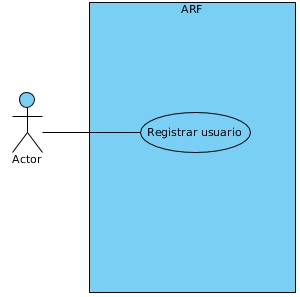
\includegraphics[width=12cm,height=6cm]{imagenes/analisis/registrarUsuario.jpg}
	\caption{Caso de uso 2 : Registrar usuario.}
	\label{fig:analogo}
\end{figure} 
\newpage
\subsection{Caso de uso 3} \textit{Gestión de muebles} \par
Escenario donde un usuario consulta, cambia de color y selecciona un mueble para visualizarlo con realidad aumentada.
\begin{figure}[h!]
	\centering
	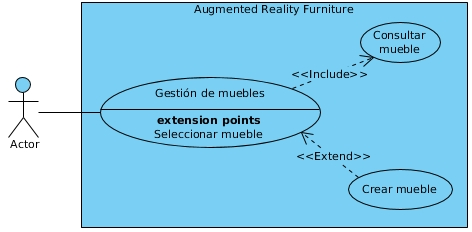
\includegraphics[width=12cm,height=6cm]{imagenes/analisis/seleccionarMueble.jpg}
	\caption{Caso de uso 3 : Gestión de muebles.}
	\label{fig:analogo}
\end{figure}

\subsection{Caso de uso 4}\textit{Crear escenario} 
\vspace{5mm}
\begin{figure}[h!]
	\centering
	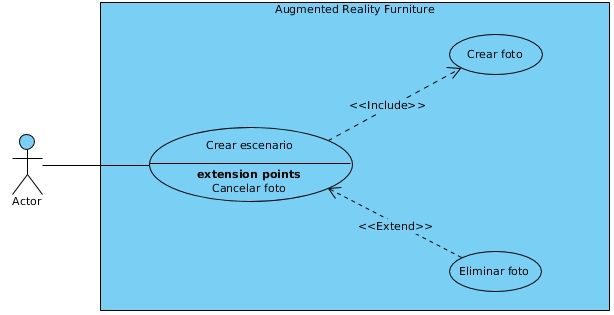
\includegraphics[width=12cm,height=6cm]{imagenes/analisis/crearEscenario.jpg}
	\caption{Crear escenario.}
	\label{fig:analogo}
\end{figure}

\subsection{Caso de uso 5}\textit{Visualizar escenario} 
\vspace{5mm}
\begin{figure}[h!]
	\centering
	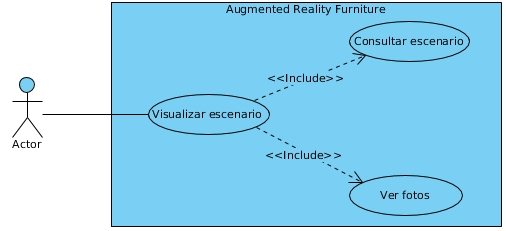
\includegraphics[width=12cm,height=6cm]{imagenes/analisis/visualizarEscenario.jpg}
	\caption{Caso de uso 5 : Visualizar escenario.}
	\label{fig:analogo}
\end{figure}